\section{Load Balancing Simulation}

The simulation feature of the load balancing framework allows the users to collect information
about the compute WALL/CPU time and communication of the chares during a particular run of
the program and use this information later to test the different load balancing strategies to
see which one is suitable for the program behavior. Currently, this feature is supported only for
the centralized load balancing strategies. For this, the load balancing framework
accepts the following command line options:
\begin{enumerate}
\item {\em +LBDump StepStart}\\
        This will dump the compute and the communication data collected by the load balancing framework
	starting from the load balancing step {\em StepStart} into a file on the disk. The name of the file
	is given by the {\em +LBDumpFile} option. The load balancing step in the
  program is numbered starting from 0. Negative value for {\em StepStart} will be converted to 0.
\item {\em +LBDumpSteps StepsNo}\\
        This option specifies the number of load balancing steps for which data will be dumped to disk.
        If omitted, default value is 1. The program will exit after {\em StepsNo} files are dumped.
\item {\em +LBDumpFile FileName}\\
        This option specifies the base name of the file created with the loadd balancing data. If this
	option is not specified, the framework uses the default file {\tt lbdata.dat}. Since multiple steps are allowed,
	a number is appended to the filename in the form {\tt Filename.\#}; this applies to both dump and
	simulation.
\item {\em +LBSim StepStart}\\
	This option instructs the framework to do the simulation from {\em StepStart} step.
	When this option is specified, the load balancing data along with the step
  number will be read from the file specified in the {\em +LBDumpFile}
	option. The program will print the results of the balancing for a number of steps given
  by the {\em +LBSimSteps} option, and then will exit.
\item {\em +LBSimSteps StepsNo}\\
        This option is applicable only to the simulation mode. It specifies the number of
  load balancing steps for which the data will be dumped. The default value is 1.
\item {\em +LBSimProcs}\\
        With this option, the user can change the number of processors
  specified to the load balancing strategy. It may be used to test
	the strategy in the cases where some processor crashes or a new processor becomes available. If this number is not
	changed since the original run, starting from the second step file the program will print other additional
	information about how the simulated load differs from the real load during the run (considering all
	strategies that were applied while running). This may be used to test the validity of a load balancer
	prediction over the reality. If the strategies used during run and simulation differ, the additional data
	printed may not be useful.
\end{enumerate}
Here is an example which collects the data for a 1000 processor run of a program
\begin{alltt}
./charmrun pgm +p1000 +balancer RandCentLB +LBDump 2 +LBDumpSteps 4 +LBDumpFile dump.dat
\end{alltt}
This will collect data on files data.dat.{2,3,4,5}. We can use this data to
analyze the performance of various centralized strategies using:
\begin{alltt}
./charmrun pgm +balancer <Strategy to test> +LBSim 2 +LBSimSteps 4 +LBDumpFile dump.dat
[+LBSimProcs 900]
\end{alltt}
Please note that this does not invoke the real application. In fact,
 ''pgm'' can be replaced with any generic application which calls centralized load balancer.
An example can be found in \testrefdir{load\_balancing/lb\_test}.

\section{Future load predictor}

When objects do not follow the assumption that the future workload will be the
same as the past, the load balancer might not have the right information to do
a good rebalancing job. To prevent this, the user can provide a transition
function to the load balancer to predict what will be the future workload, given
the past, instrumented one. For this, the user can provide a specific class
which inherits from {\tt LBPredictorFunction} and implement the appropriate functions. 
Here is the abstract class:
\begin{alltt}
class LBPredictorFunction \{
public:
  int num_params;
 
  virtual void initialize_params(double *x);

  virtual double predict(double x, double *params) =0;
  virtual void print(double *params) {PredictorPrintf("LB: unknown model");};
  virtual void function(double x, double *param, double &y, double *dyda) =0;
\};
\end{alltt}
\begin{itemize}
\item {\tt initialize\_params} by default initializes the parameters randomly. If the user
knows how they should be, this function can be re-implemented.
\item {\tt predict} is the function that predicts the based on the function parameters.
An example for the {\em predict} function is given below.
\begin{verbatim}
double predict(double x, double *param) {return (param[0]*x + param[1]);}
\end{verbatim}
\item {\tt print} is useful for debugging and it can be re-implemented to have a meaningful
print of the learnt model
\item {\tt function} is a function internally needed to learn the parameters, {\tt x} and
{\tt param} are input, {\tt y} and {\tt dyda} are output (the computed function and
all its derivatives with respect to the parameters, respectively).
For the function in the example should look like:
\begin{verbatim}
void function(double x, double *param, double &y, double *dyda) {
  y = predict(x, param);
  dyda[0] = x;
  dyda[1] = 1;
}
\end{verbatim}
\end{itemize}
Other than these functions, the user should provide a constructor which must initialize
{\tt num\_params} to the number of parameters the model has to learn. This number is
the dimension of {\tt param} and {\tt dyda} in the previous functions. For the given
example, the constructor is {\tt \{num\_params = 2;\}}.

If the model for computation is not known, the user can leave the system to
use the default function.

As seen, the function can have several parameters which will be learned during
the execution of the program. For this, two parameters can be setup at command
line to specify the learning behavior:
\begin{enumerate}
\item {\em +LBPredictorWindow size}\\
This parameter specifies the number of statistics steps the load balancer will
store.  The greater this number is, the better the
approximation of the workload will be, but more memory is required to store
the intermediate information. The default is 20.
\item {\em +LBPredictorDelay steps}\\
This will tell how many load balancer steps to wait before considering the
function parameters learnt and starting to use the mode. The load balancer will
collect statistics for a {\em +LBPredictorWindow} steps, but it will start using
the model as soon as {\em +LBPredictorDelay} information are collected. The
default is 10.
\end{enumerate}
Moreover another flag can be set to enable the predictor from command line: {\em
+LBPredictor}.\\
Other than the command line options, there are some methods
which can be called from the user program to modify the predictor. These methods are:
\begin{itemize}
\item {\tt void PredictorOn(LBPredictorFunction *model);}
\item {\tt void PredictorOn(LBPredictorFunction *model,int wind);}
\item {\tt void PredictorOff();}
\item {\tt void ChangePredictor(LBPredictorFunction *model);}
\end{itemize}

\section{Control CPU Load Statistics}

\charmpp{} programmers can control CPU load data in the load balancing database
before a load balancing phase starts (which is the time when load balancing
database is collected and used by load balancing strategies).

In an array element, the following function can be invoked to overwrite the 
CPU load that is measured by the load balancing framework.

\begin{alltt}
   double newTiming;
   setObjTime(newTiming);
\end{alltt}

{\em setObjTime()} is defined as a method of class {\em CkMigratable}, which is
the superclass of all array elements.

The users can also retrieve the current timing that the load balancing runtime
has measured for the current array element. 
 
\begin{alltt} 
   double measuredTiming; 
   measuredTiming = getObjTime(); 
\end{alltt}

This is useful when the users want to derive a new CPU load based on the 
existing one.

\section{Model-based Load Balancing}

The user can choose to feed load balancer with their own CPU
timing of each Chare based on certain computational model of the applications.

To do so, the user first needs to turn off automatic CPU load measurement completely
by setting:

\begin{alltt}
   usesAutoMeasure = CmiFalse;
\end{alltt}

in array element's constructor.

The user must also implement the following function to the chare array
classes:

\begin{alltt}
   virtual void CkMigratable::UserSetLBLoad();      // defined in base class
\end{alltt}

This function serves as a callback that is called on each chare object when
{\em AtSync()} is called and ready to do load balancing. The implementation of
{\em UserSetLBLoad()} is simply to set the current chare object's CPU load in
load balancing framework. {\em setObjTime()} described above can be used for
this.

\section{Writing a new load balancing strategy}

\charmpp{} programmers can choose an existing load balancing strategy from
\charmpp{}'s built-in strategies(see ~\ref{lbStrategy}) for the best performance
based on the characteristics of their applications. However, they can also
choose to write their own load balancing strategies.

The \charmpp{} load balancing framework provides a simple scheme to incorporate
new load balancing strategies. The programmer needs to write their strategy for
load balancing based on the instrumented ProcArray and ObjGraph provided by the
load balancing framework. This strategy is implemented within this
function:

\begin{alltt}
void FooLB::work(LDStats *stats) \{
  /** ========================== INITIALIZATION ============================= */
  ProcArray *parr = new ProcArray(stats);
  ObjGraph *ogr = new ObjGraph(stats);

  /** ============================= STRATEGY ================================ */
  /// The strategy goes here
  /// The strategy goes here
  /// The strategy goes here
  /// The strategy goes here
  /// The strategy goes here

  /** ============================== CLEANUP ================================ */
  ogr->convertDecisions(stats);
\}
\end{alltt}

Figure~\ref{fig:ckgraph} explains the two data structures available to the
strategy: ProcArray and ObjGraph. Using them, the strategy should assign objects 
to new processors  where it wants to be migrated through the setNewPe() method.
{\tt src/ck-ldb/GreedyLB.C} can be referred.
\begin{figure}[h]
\centering
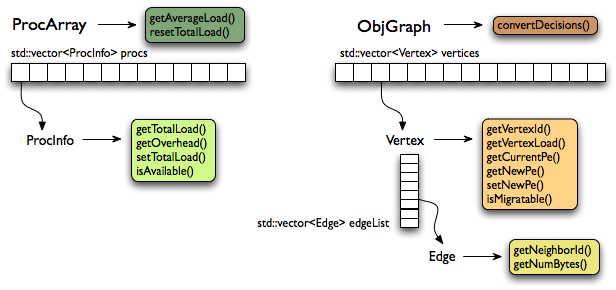
\includegraphics[width=6.0in]{fig/ckgraph.png}
\caption{ProcArray and ObjGraph data structures to be used when writing a load
balancing strategy}
\label{fig:ckgraph}
\end{figure}

Incorporating this strategy into the \charmpp{} build framework is explained in
the next section.

\section{Adding a load balancer to \charmpp{}}

Let us assume that we are writing a new centralized load balancer called FooLB.
The next few steps explain the steps of adding the load balancer to the \charmpp{}
build system:

\begin{enumerate}
\item Create files named {\em FooLB.ci, FooLB.h and FooLB.C} in directory of {\tt src/ck-ldb}.
One can choose to copy and rename the files GraphPartLB.* and rename the class name in those
files.

\item Implement the strategy in the {\em FooLB} class method --- {\bf
FooLB::work(LDStats* stats)} as described in the previous section.
%This method takes the load balancing database ({\em stats}) as an input, and
%output the new mapping of objects to processors in {\em stats->to\_proc}
%array.

\item Build charm for your platform (This will create the required links in the
tmp directory).

\item To compile the strategy files, first add {\em FooLB} in the ALL\_LDBS
list in charm/tmp/Makefile\_lb.sh. Also comment out the line containing
UNCOMMON\_LDBS in Makefile\_lb.sh.  If FooLB will require some libraries at
link time, you also need to create the dependency file called
libmoduleFooLB.dep. Run the script in charm/tmp, which creates the new Makefile
named ``Make.lb''.

\item Run ``make depends'' to update dependence rule of \charmpp{} files.  And run
``make charm++'' to compile \charmpp{} which includes the new load balancing
strategy files.
\end{enumerate}


\section{Understand Load Balancing Database Data Structure}
\label{lbdatabase}

To write a load balancing strategy, you need to know 
what information is measured during the runtime and how it is represented in
the load balancing database data structure.

There are mainly 3 categories of information: a) processor information including processor speed, background load; b) object information including per object
CPU/WallClock compute time and c) communication information .

The database data structure named {\kw LDStats} is defined in {\em CentralLB.h}:

\begin{verbatim}

  struct ProcStats {  // per processor
    LBRealType total_walltime;
    LBRealType total_cputime;
    LBRealType idletime;
    LBRealType bg_walltime;
    LBRealType bg_cputime;
    int pe_speed;
    double utilization;
    CmiBool available;
    int   n_objs;
  }

  struct LDStats { // load balancing database
    ProcStats  *procs;
    int count;

    int   n_objs;
    int   n_migrateobjs;
    LDObjData* objData;

    int   n_comm;
    LDCommData* commData;

    int  *from_proc, *to_proc;
  }

\end{verbatim}

\begin{enumerate}
\item {\em LBRealType} is the data type for load balancer measured time. It is "double" by default. User can specify the type to float at \charmpp{} compile time if want. For example, ./build charm++ net-linux-x86\_64 {-}{-}with-lbtime-type=float;
\item {\em procs} array defines processor attributes and usage data for each
processor;
\item {\em objData} array records per object information, {\em LDObjData} is defined in {\em lbdb.h};
\item {\em commData} array records per communication information. {\em LDCommData} is defined in {\em lbdb.h}.
\end{enumerate}

